% THIS DOCUMENT IS TAILORED TO REQUIREMENTS FOR SCIENTIFIC COMPUTING.  IT SHOULDN'T
% BE USED FOR NON-SCIENTIFIC COMPUTING PROJECTS
\documentclass[12pt]{article}

\usepackage{amsmath, mathtools}
\usepackage{amsfonts}
\usepackage{amssymb}
\usepackage{graphicx}
\usepackage{colortbl}
\usepackage{xr}
\usepackage{hyperref}
\usepackage{longtable}
\usepackage{xfrac}
\usepackage{tabularx}
\usepackage{float}
\usepackage{siunitx}
\usepackage{booktabs}
\usepackage{caption}
\usepackage{pdflscape}
\usepackage{afterpage}
\usepackage{svg}

\usepackage[round]{natbib}

%\usepackage{refcheck}

\hypersetup{
    bookmarks=true,         % show bookmarks bar?
      colorlinks=true,       % false: boxed links; true: colored links
    linkcolor=red,          % color of internal links (change box color with linkbordercolor)
    citecolor=green,        % color of links to bibliography
    filecolor=magenta,      % color of file links
    urlcolor=cyan           % color of external links
}

\input{../Comments}
%% Common Parts

\newcommand{\progname}{2D-RAPP} % PUT YOUR PROGRAM NAME HERE
\newcommand{\authname}{Ziyang(Ryan) Fang} % AUTHOR NAMES                  

\usepackage{hyperref}
    \hypersetup{colorlinks=true, linkcolor=blue, citecolor=blue, filecolor=blue,
                urlcolor=blue, unicode=false}
    \urlstyle{same}
                                


% For easy change of table widths
\newcommand{\colZwidth}{1.0\textwidth}
\newcommand{\colAwidth}{0.13\textwidth}
\newcommand{\colBwidth}{0.82\textwidth}
\newcommand{\colCwidth}{0.1\textwidth}
\newcommand{\colDwidth}{0.05\textwidth}
\newcommand{\colEwidth}{0.8\textwidth}
\newcommand{\colFwidth}{0.17\textwidth}
\newcommand{\colGwidth}{0.5\textwidth}
\newcommand{\colHwidth}{0.28\textwidth}

% Used so that cross-references have a meaningful prefix
\newcounter{defnum} %Definition Number
\newcommand{\dthedefnum}{GD\thedefnum}
\newcommand{\dref}[1]{GD\ref{#1}}
\newcounter{datadefnum} %Datadefinition Number
\newcommand{\ddthedatadefnum}{DD\thedatadefnum}
\newcommand{\ddref}[1]{DD\ref{#1}}
\newcounter{theorynum} %Theory Number
\newcommand{\tthetheorynum}{TM\thetheorynum}
\newcommand{\tref}[1]{TM\ref{#1}}
\newcounter{tablenum} %Table Number
\newcommand{\tbthetablenum}{TB\thetablenum}
\newcommand{\tbref}[1]{TB\ref{#1}}
\newcounter{assumpnum} %Assumption Number
\newcommand{\atheassumpnum}{A\theassumpnum}
\newcommand{\aref}[1]{A\ref{#1}}
\newcounter{goalnum} %Goal Number
\newcommand{\gthegoalnum}{GS\thegoalnum}
\newcommand{\gsref}[1]{GS\ref{#1}}
\newcounter{instnum} %Instance Number
\newcommand{\itheinstnum}{IM\theinstnum}
\newcommand{\iref}[1]{IM\ref{#1}}
\newcounter{reqnum} %Requirement Number
\newcommand{\rthereqnum}{R\thereqnum}
\newcommand{\rref}[1]{R\ref{#1}}
\newcounter{nfrnum} %NFR Number
\newcommand{\rthenfrnum}{NFR\thenfrnum}
\newcommand{\nfrref}[1]{NFR\ref{#1}}
\newcounter{lcnum} %Likely change number
\newcommand{\lthelcnum}{LC\thelcnum}
\newcommand{\lcref}[1]{LC\ref{#1}}

\usepackage{fullpage}

\newcommand{\deftheory}[9][Not Applicable]
{
\newpage
\noindent \rule{\textwidth}{0.5mm}

\paragraph{RefName: } \textbf{#2} \phantomsection 
\label{#2}

\paragraph{Label:} #3

\noindent \rule{\textwidth}{0.5mm}

\paragraph{Equation:}

#4

\paragraph{Description:}

#5

\paragraph{Notes:}

#6

\paragraph{Source:}

#7

\paragraph{Ref.\ By:}

#8

\paragraph{Preconditions for \hyperref[#2]{#2}:}
\label{#2_precond}

#9

\paragraph{Derivation for \hyperref[#2]{#2}:}
\label{#2_deriv}

#1

\noindent \rule{\textwidth}{0.5mm}

}

\begin{document}

\title{Software Requirements Specification for 2D Robot Arms for Path Planning} 
\author{\ Ziyang(Ryan) Fang}
\date{\today}
	
\maketitle

~\newpage

\pagenumbering{roman}

\tableofcontents

~\newpage

\section*{Revision History}

\begin{tabularx}{\textwidth}{p{3cm}p{2cm}X}
\toprule {\bf Date} & {\bf Version} & {\bf Notes}\\
\midrule
Feb 02 2025 & 1.0 & Notes\\
% Date 2 & 1.1 & Notes\\
\bottomrule
\end{tabularx}

~\\
\plt{This template is intended for use by CAS 741.  For CAS 741 the template
should be used exactly as given, except the Reflection Appendix can be deleted.
For the capstone course it is a source of ideas, but shouldn't be followed
exactly.  The exception is the reflection appendix.  All capstone SRS documents
should have a reflection appendix.}

~\newpage

\section{Reference Material}

This section records information for easy reference.

\subsection{Table of Units}

Throughout this document SI (Syst\`{e}me International d'Unit\'{e}s) is employed
as the unit system.  In addition to the basic units, several derived units are
used as described below.  For each unit, the symbol is given followed by a
description of the unit and the SI name.
~\newline

\renewcommand{\arraystretch}{1.2}
  \noindent \begin{tabular}{l l l} 
    \toprule		
    \textbf{symbol} & \textbf{unit} & \textbf{SI}\\
    \midrule 
    \si{\centi\metre} & length & centimetre \\
    % \si{\kilogram} & mass & kilogram \\
    \si{\second} & time & second \\
    \( q \) & joint angle & radians \\
    \(\dot{q}\) & joint velocity & rad/s \\
    \(\ddot{q}\) & joint acceleration & rad/s² \\
    % \si{\newton\metre} & torque & newton metre \\
    \bottomrule
  \end{tabular}
  %	\caption{Provide a caption}
%\end{table}

\plt{Only include the units that your SRS actually uses.}

\plt{Derived units, like newtons, pascal, etc, should show their derivation
    (the units they are derived from) if their constituent units are in the
    table of units (that is, if the units they are derived from are used in the
    document).  For instance, the derivation of pascals as
    $\si{\pascal}=\si{\newton\per\square\meter}$ is shown if newtons and m are
    both in the table.  The derivations of newtons would not be shown if kg and
    s are not both in the table.}

\plt{The symbol for units named after people use capital letters, but the name
  of the unit itself uses lower case.  For instance, pascals use the symbol Pa,
  watts use the symbol W, teslas use the symbol T, newtons use the symbol N,
  etc.  The one exception to this is degree Celsius.  Details on writing metric
  units can be found on the 
  \href{https://www.nist.gov/pml/weights-and-measures/writing-metric-units}
  {NIST} web-page.}

\subsection{Table of Symbols}

The table that follows summarizes the symbols used in this document along with
their units.  The choice of symbols was made to be consistent with the heat
transfer literature and with existing documentation for solar water heating
systems.  The symbols are listed in alphabetical order.

\renewcommand{\arraystretch}{1.2}
%\noindent \begin{tabularx}{1.0\textwidth}{l l X}
\noindent \begin{longtable*}{l l p{12cm}} \toprule
\textbf{symbol} & \textbf{unit} & \textbf{description}\\
\midrule 
\( L \) & \si{\centi\metre} & Link length of the robot arm \\
\( q \) & radians & Joint angle \\
\( \dot{q} \) & rad/s & Joint angular velocity \\
\( \ddot{q} \) & rad/s² & Joint angular acceleration \\
\( x, y \) & \si{\centi\metre} & Cartesian coordinates of the end-effector \\
\( T \) & \si{\second} & Total time for motion execution \\
\( t \) & \si{\second} & Time step \\
\( \mathbf{q}_{\text{init}} \) & radians & Initial joint configuration \\
\( \mathbf{q}_{\text{goal}} \) & radians & Goal joint configuration \\
\( O_i \) & \si{\centi\metre} & Position of the \(i\)-th obstacle (circular) \\
\( r_i \) & \si{\centi\metre} & Radius of the \(i\)-th obstacle \\
\( M \) & - & Number of discrete joint positions in A* search grid \\
\( \theta_i \) & radians & Discretized joint angle for A* search \\
\( \mathcal{G} \) & - & Occupancy grid (joint space) \\
\( \mathbf{p}_i \) & \si{\centi\metre} & Position of the \(i\)-th joint \\

\bottomrule
\end{longtable*}


\subsection{Abbreviations and Acronyms}

\renewcommand{\arraystretch}{1.2}
\begin{tabular}{l l} 
  \toprule		
  \textbf{symbol} & \textbf{description}\\
  \midrule 
  A & Assumption\\
  DD & Data Definition\\
  GD & General Definition\\
  GS & Goal Statement\\
  IM & Instance Model\\
  LC & Likely Change\\
  PS & Physical System Description\\
  R & Requirement\\
  SRS & Software Requirements Specification\\
  TM & Theoretical Model\\
  IK & Inverse Kinematics \\
  FK & Forward Kinematics \\
  A* & A-star Pathfinding Algorithm \\
  DOF & Degrees of Freedom \\
  EE & End-Effector \\
  % \progname{} & 2DPL\\
  TM & Theoretical Model\\
  2D-RAPP & 2D Robot Arm Path Planning\\
  \bottomrule
\end{tabular}\\

\plt{Add any other abbreviations or acronyms that you add}



\section{Introduction}
Path planning for robotic manipulators is a fundamental problem in robotics, enabling robots to move efficiently and safely within constrained environments. Unlike mobile robots that navigate in free space, robotic arms must operate in a higher-dimensional joint space, where each degree of freedom contributes to the overall complexity of motion planning. Traditional inverse kinematics (IK) methods solve for joint angles that satisfy end-effector goals, but they often struggle with obstacle avoidance and computational efficiency in real-time applications.

This document provides an overview of the Software Requirements Specification (SRS) for a 2D robotic arm path planning system based on a graph-based inverse kinematics (IK) approach with A* search. The developed program will be referred to as 2D Robot Arm Path Planning (2D-RAPP) throughout this document. This section explains the purpose of this document, the scope of the requirements, the characteristics of the intended reader, and the organization of the document.

\subsection{Purpose of Document}
The primary purpose of this document is to record the requirements of 2D-RAPP. Goals, assumptions, theoretical models, definitions, and other derivation information are specified, allowing the reader to fully understand and verify the purpose and scientific basis of 2D-RAPP. With the exception of system constraints, this SRS remains abstract, describing what problem is being solved, but not how to solve it.

This document serves as a starting point for subsequent development phases, including writing the design specification and the software verification and validation plan. The design document will show how the requirements are to be realized, including decisions on numerical algorithms, data structures, and programming frameworks. The verification and validation plan will outline the steps required to increase confidence in the software’s correctness, reliability, and performance. 

Although this SRS follows a structured documentation approach, it does not impose any specific software development methodology. Regardless of whether a waterfall, agile, or iterative development process is followed, it remains useful to present the documentation in a way that maintains clarity and logical structure, as recommended by Parnas and Clements.



\subsection{Scope of Requirements} 
The scope of the requirements includes path planning for a 2D robotic arm with N revolute joints, operating in a workspace with circular obstacles. The system is designed to compute collision-free paths in joint space, using distance-based inverse kinematics and search algorithms.


\subsection{Characteristics of Intended Reader} \label{sec_IntendedReader}
Reviewers of this documentation should have a fundamental understanding of robotics kinematics at an undergraduate level, specifically covering forward kinematics, inverse kinematics, and path planning. Familiarity with graph-based search algorithms (such as A*) and numerical optimization techniques is also recommended.

The users of 2D-RAPP (e.g., robotics researchers, engineers) may have varying levels of expertise, as explained in Section~\ref{SecUserCharacteristics}. However, those involved in **reviewing, modifying, or maintaining this SRS** should have a **strong background in computational kinematics and algorithmic path planning**.


\subsection{Organization of Document}

This document follows the standard structure of an SRS for scientific computing software. It begins with the problem statement and goals, followed by theoretical foundations, definitions, and assumptions. The document then presents instance models and specific requirements.

The problem is introduced through kinematic models and path planning techniques, including forward and inverse kinematics and graph-based search methods. Assumptions related to joint constraints and obstacle avoidance are also outlined.

Readers can approach this document either top-down, starting from goals to implementation, or bottom-up, beginning with instance models and tracing back to theoretical foundations. The instance model IM:PathPlanning defines the core algorithm for collision-free motion planning of a 2D robot arm.


\section{General System Description}

This section provides general information about the system.  It identifies the
interfaces between the system and its environment, describes the user
characteristics and lists the system constraints. 


\subsection{System Context}


Fig.~\ref{Fig:SysCon} illustrates the system context. The circle represents the user, an external entity providing inputs to the system. The rectangle represents the software system, 2D-RAPP. Arrows indicate the data flow between the user and the system.

\begin{figure}[h!]
\centering
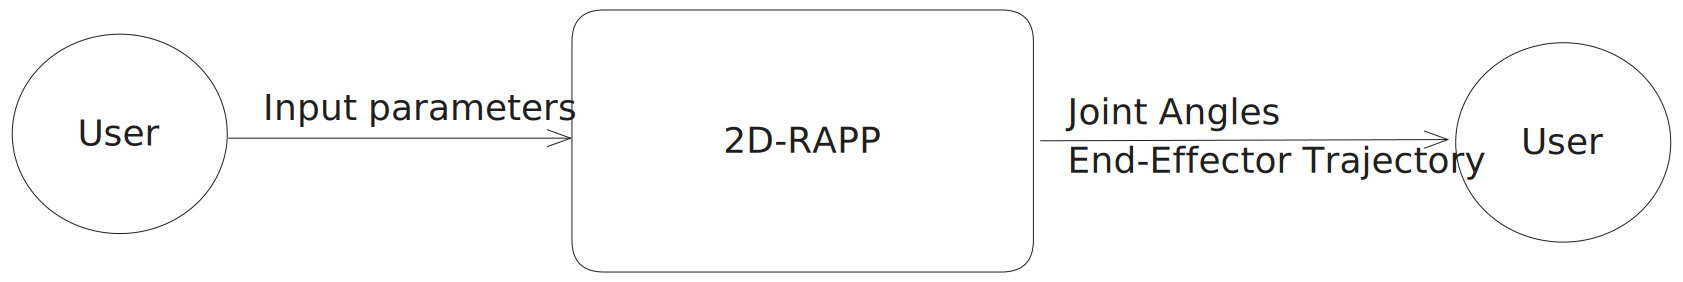
\includegraphics[width=0.8\textwidth]{SystemContextFigure}
\caption{System Context}
\label{Fig:SysCon}
\end{figure}

The interaction between the user and the system is described as follows:

\subsubsection*{User Responsibilities}
\begin{itemize}
    \item Provide the input data to the system, including:
    \begin{itemize}
        \item Initial joint angles (\(q_{\text{init}}\)) to specify the starting configuration of the robotic arm.
        \item Goal position (\(x_{\text{goal}}, y_{\text{goal}}\)) to indicate the desired end-effector target.
        \item Obstacle data, including radii (\(r_i\)) and positions (\(O_i = (x_i, y_i)\)).
    \end{itemize}
    \item Ensure the input data is accurate and in the required units.
\end{itemize}

\subsubsection*{2D-RAPP Responsibilities}
\begin{itemize}
    \item Detect input errors, such as invalid data types or inconsistent units.
    \item Verify that the inputs satisfy physical and software constraints.
    \item Compute a collision-free trajectory for the robotic arm, including:
    \begin{itemize}
        \item Joint angles (\(q\), \(\dot{q}\), \(\ddot{q}\)) for each motion stage.
        \item Cartesian path (\(x, y\)) of the end-effector.
    \end{itemize}
    \item Provide a visual representation of the robotic arm's movement and obstacle avoidance.
\end{itemize}

This system context defines the roles and interactions between the user and the 2D-RAPP system, ensuring clarity in the data flow and system responsibilities.


\subsection{User Characteristics} \label{SecUserCharacteristics}
The intended users of \progname{} are individuals with a background in robotics, computer science, and mechanical engineering. They are expected to have a fundamental understanding of kinematics, particularly inverse kinematics, and be familiar with basic path planning algorithms. 


\subsection{System Constraints}
There are no system constraints.


\section{Specific System Description}

This section first presents the problem description, which gives a high-level
view of the problem to be solved.  This is followed by the solution characteristics
specification, which presents the assumptions, theories, definitions and finally
the instance models. The system focuses on generating a collision-free trajectory for a 2D robotic arm in an environment with static obstacles. The robotic arm is modeled as a serial manipulator with revolute joints, and its configuration is defined by a set of joint angles.


\subsection{Problem Description} \label{Sec_pd}

\progname{} is intended to solve the path planning for 2D robotic arms.



\subsubsection{Terminology and  Definitions}


This subsection provides a list of terms that are used in the subsequent
sections and their meaning, with the purpose of reducing ambiguity and making it
easier to correctly understand the requirements:

\begin{itemize}

  \item \textbf{Joint space:} The space defined by the possible values of the robot arm’s joint angles.
  
  \item \textbf{Workspace:} The Cartesian space where the end-effector of the robotic arm can reach.
  
  \item \textbf{Obstacle:} A static circular object in the workspace that the robotic arm must avoid.
  
  \item \textbf{Trajectory:} A sequence of joint configurations representing a smooth motion of the robotic arm from the start to the goal.
  
  \item \textbf{Configuration:} A specific set of joint angles that fully describes the position of the robotic arm.
  
  \item \textbf{Collision detection:} The process of determining whether the robotic arm intersects with an obstacle.
  
  \item \textbf{Path planning:} The process of computing a collision-free sequence of configurations to move the robotic arm from the start to the goal.
  
  \item \textbf{Inverse kinematics:} The process of determining joint angles given a desired end-effector position.
  
  \item \textbf{Forward kinematics:} The computation of the end-effector position given joint angles.
  
  \end{itemize}

\subsubsection{Physical System Description} \label{sec_phySystDescrip}


The physical system of \progname{}, as shown in Figure~\ref{Fig:Robotic arm},
includes the following elements:

\begin{itemize}

  \item[PS1:] A robotic arm with two revolute joints, defining a two-link planar mechanism.
  
  \item[PS2:] The environment contains static circular obstacles that must be avoided by the arm.
  
  \item[PS3:] A discretized joint space where joint angles are sampled uniformly to form a toroidal search space.
  
  \item[PS4:] A start configuration that represents the initial joint angles of the robotic arm.
  
  \item[PS5:] A goal configuration that represents the desired joint angles to reach the target position.
  
  \item[PS6:] The A* algorithm used to compute the shortest collision-free path in joint space.
  
  \end{itemize}


\begin{figure}[h!]
\begin{center}
%\rotatebox{-90}
{
 \includegraphics[width=0.5\textwidth]{Physical System Description}
}
\caption{Robotic arm finding a path to target point}
\label{Fig:Robotic arm} 
\end{center}
\end{figure}

\subsubsection{Goal Statements}

\noindent Given the initial joint angles, the goal joint angles, and the obstacle locations, the goal statements are:

\begin{itemize}

\item[GS\refstepcounter{goalnum}\thegoalnum \label{GS_CollisionFreePath}:] Compute a collision-free trajectory in joint space from the start configuration to the goal configuration.

\item[GS\refstepcounter{goalnum}\thegoalnum \label{GS_OptimizePath}:] Minimize the total path length while ensuring obstacle avoidance.

\item[GS\refstepcounter{goalnum}\thegoalnum \label{GS_SmoothMotion}:] Generate a smooth and continuous motion trajectory for the robotic arm.

\item[GS\refstepcounter{goalnum}\thegoalnum \label{GS_PathSafety}:] Validate the safety of the planned path by verifying obstacle-free movement at each configuration.

\end{itemize}

\subsection{Solution Characteristics Specification}

The instance models that govern \progname{} are presented in the Instance Model Section. The necessary information to understand the meaning of the instance models and their derivation is also included, ensuring that the instance models can be verified. The solution characteristics describe the assumptions, theoretical foundations, and mathematical formulations that define the problem space and provide a basis for trajectory planning and obstacle avoidance in robotic arm motion.


\begin{figure}[H]
  \includegraphics[scale=0.9]{RelationsBetweenTM_GD_IM_DD_A.pdf}
\end{figure}

The instance models that govern \progname{} are presented in
Subsection~\ref{sec_instance}.  The information to understand the meaning of the
instance models and their derivation is also presented, so that the instance
models can be verified.

\subsubsection{Assumptions} \label{sec_assumpt}


This section simplifies the original problem and helps in developing the
theoretical model by filling in the missing information for the physical system.
The numbers given in the square brackets refer to the theoretical model [TM],
general definition [GD], data definition [DD], instance model [IM], or likely
change [LC], in which the respective assumption is used.

\begin{itemize}

  \item[A\refstepcounter{assumpnum}\theassumpnum \label{A_KinematicMotionOnly}:] 
  The motion of the robotic arm is modeled purely kinematically, without considering the effects of dynamics such as forces, torques, or friction. (RefBy: IM:PathPlanning)

\item[A\refstepcounter{assumpnum}\theassumpnum \label{A_LinkLengthsConstant}:] 
  The lengths of all links in the robotic arm are constant and do not change during motion. (RefBy: GD:ForwardKinematics)

\item[A\refstepcounter{assumpnum}\theassumpnum \label{A_JointMotionContinuous}:] 
  The joint angles of the robotic arm vary smoothly and continuously without sudden jumps. (RefBy: IM:TrajectoryGeneration)

\item[A\refstepcounter{assumpnum}\theassumpnum \label{A_NoMechanicalDeflection}:] 
  The robotic arm links are considered rigid, meaning there is no mechanical deflection or deformation. (RefBy: GD:InverseKinematics)

\item[A\refstepcounter{assumpnum}\theassumpnum \label{A_ObstacleShapeCircular}:] 
  Obstacles in the environment are approximated as circles with predefined radii. (RefBy: IM:CollisionDetection)

\item[A\refstepcounter{assumpnum}\theassumpnum \label{A_TrajectoryDiscretized}:] 
  The planned trajectory is discretized into a series of intermediate waypoints in joint space. (RefBy: IM:TrajectoryGeneration)

\item[A\refstepcounter{assumpnum}\theassumpnum \label{A_InitialAndGoalConfigurationsKnown}:] 
  The initial joint configuration and the goal joint configuration are known before path planning begins. (RefBy: IM:PathPlanning)

\end{itemize}

\subsubsection{Theoretical Models}\label{sec_theoretical}

This section focuses on the general equations and laws that \progname{} is based
on. The theoretical models serve as fundamental principles governing the kinematic motion and path planning of the robotic arm. 

~\newline

\noindent
\deftheory
% #2 refname of theory
{TM:FWDKinematics}
% #3 label
{Forward Kinematics}
% #4 equation
{
  $\mathbf{x} = f(\mathbf{q}) = \begin{bmatrix}
  L_1 \cos(\theta_1) + L_2 \cos(\theta_1 + \theta_2) \\
  L_1 \sin(\theta_1) + L_2 \sin(\theta_1 + \theta_2)
  \end{bmatrix}$
}
% #5 description
{
  \begin{itemize}
    \item $\mathbf{q}$: Joint angles, where $\theta_1$ is the angle of the first joint and $\theta_2$ is the relative angle of the second joint.
    \item $L_1$: Length of the first link (\si{\centi\metre}).
    \item $L_2$: Length of the second link (\si{\centi\metre}).
  \end{itemize}
}
% #6 Notes
{
  This forward kinematics model assumes:
  \begin{itemize}
    \item Rigid links: The links are assumed to be perfectly rigid and do not deform under load (\aref{A_LinkLengthsConstant}).
    \item Fixed base: The base of the arm is considered stationary, located at the origin $(0, 0)$.
    \item Ideal joints: The joints rotate without friction or other physical limitations.
    \item Planar motion: The arm operates in a 2D plane, and there is no out-of-plane movement.
  \end{itemize}

  These assumptions ensure simplicity and accuracy for theoretical modeling. For real-world applications, additional factors such as joint compliance, link flexibility, and external forces may need to be considered.
}
% #7 Source
{
  \url{https://atsushisakai.github.io/PythonRobotics/modules/7_arm_navigation/planar_two_link_ik.html}
}
% #8 Referenced by
{
  \dref{ROCT}
}
% #9 Preconditions
{
None
}
% #1 derivation - not applicable by default
{}

\plt{``Ref.\ By'' is used repeatedly with the different types of information.
  This stands for Referenced By.  It means that the models, definitions and
  assumptions listed reference the current model, definition or assumption.
  This information is given for traceability.  Ref. By provides a pointer in the
  opposite direction to what we commonly do.  You still need to have a reference
  in the other direction pointing to the current model, definition or
  assumption.  As an example, if TM1 is referenced by GD2, that means that GD2 will
  explicitly include a reference to TM1.}

~\newline

\subsubsection{General Definitions}\label{sec_gendef}

\plt{General Definitions (GDs) are a refinement of one or more TMs, and/or of
  other GDs.  The GDs are less abstract than the TMs.  Generally the reduction
  in abstraction is possible through invoking (using/referencing) Assumptions.
  For instance, the TM could be Newton's Law of Cooling stated abstracting.  The
  GD could take the general law and apply it to get a 1D equation.}

This section collects the laws and equations that will be used in building the
instance models.

\plt{Some projects may not have any content for this section, but the section
  heading should be kept.}  \plt{Modify the examples below for your problem, and
  add additional definitions as appropriate.}

~\newline

\noindent
\begin{minipage}{\textwidth}
\renewcommand*{\arraystretch}{1.5}
\begin{tabular}{| p{\colAwidth} | p{\colBwidth}|}
\hline
\rowcolor[gray]{0.9}
Number& GD\refstepcounter{defnum}\thedefnum \label{NL}\\
\hline
Label &\bf Newton's law of cooling \\
\hline
% Units&$MLt^{-3}T^0$\\
% \hline
SI Units&\si{\watt\per\square\metre}\\
\hline
Equation&$ q(t) = h \Delta T(t)$  \\
\hline
Description &
Newton's law of cooling describes convective cooling from a surface.  The law is
stated as: the rate of heat loss from a body is proportional to the difference
in temperatures between the body and its surroundings.
\\
& $q(t)$ is the thermal flux (\si{\watt\per\square\metre}).\\
& $h$ is the heat transfer coefficient, assumed independent of $T$ (\aref{A_hcoeff})
	(\si{\watt\per\square\metre\per\celsius}).\\
&$\Delta T(t)$= $T(t) - T_{\text{env}}(t)$ is the time-dependent thermal gradient
between the environment and the object (\si{\celsius}).
\\
\hline
  Source & Citation here \\
  \hline
  Ref.\ By & \ddref{FluxCoil}, \ddref{FluxPCM}\\
  \hline
\end{tabular}
\end{minipage}\\

\subsubsection*{Detailed derivation of simplified rate of change of temperature}

\plt{This may be necessary when the necessary information does not fit in the
  description field.}
\plt{Derivations are important for justifying a given GD.  You want it to be
  clear where the equation came from.}

\subsubsection{Data Definitions}\label{sec_datadef}

\plt{The Data Definitions are definitions of symbols and equations that are
  given for the problem.  They are not derived; they are simply used by other
  models.  For instance, if a problem depends on density, there may be a data
  definition for the equation defining density.  The DDs are given information
  that you can use in your other modules.}

\plt{All Data Definitions should be used (referenced) by at least one other
  model.}

This section collects and defines all the data needed to build the instance
models. The dimension of each quantity is also given.  \plt{Modify the examples
  below for your problem, and add additional definitions as appropriate.}

~\newline

\noindent
\begin{minipage}{\textwidth}
\renewcommand*{\arraystretch}{1.5}
\begin{tabular}{| p{\colAwidth} | p{\colBwidth}|}
\hline
\rowcolor[gray]{0.9}
Number& DD\refstepcounter{datadefnum}\thedatadefnum \label{FluxCoil}\\
\hline
Label& \bf Heat flux out of coil\\
\hline
Symbol &$q_C$\\
\hline
% Units& $Mt^{-3}$\\
% \hline
  SI Units & \si{\watt\per\square\metre}\\
  \hline
  Equation&$q_C(t) = h_C (T_C - T_W(t))$, over area $A_C$\\
  \hline
  Description & 
                $T_C$ is the temperature of the coil (\si{\celsius}).  $T_W$ is the temperature of the water (\si{\celsius}).  
                The heat flux out of the coil, $q_C$ (\si{\watt\per\square\metre}), is found by
                assuming that Newton's Law 
                of Cooling applies (\aref{A_Newt_coil}).  This law (\dref{NL}) is used on the surface of
                the coil, which has area $A_C$ (\si{\square\metre}) and heat 
                transfer coefficient $h_C$
                (\si{\watt\per\square\metre\per\celsius}).  This equation
                assumes that the temperature of the coil is constant over time (\aref{A_tcoil}) and that it does not vary along the length
                of the coil (\aref{A_tlcoil}).
  \\
  \hline
  Sources& Citation here \\
  \hline
  Ref.\ By & \iref{ewat}\\
  \hline
\end{tabular}
\end{minipage}\\

\subsubsection{Data Types}\label{sec_datatypes}

\plt{This section is optional.  In many scientific computing programs it isn't
  necessary, since the inputs and outpus are straightforward types, like reals,
  integers, and sequences of reals and integers.  However, for some problems it
  is very helpful to capture the type information.}

\plt{The data types are not derived; they are simply stated and used by other
  models.}

\plt{All data types must be used by at least one of the models.}

\plt{For the mathematical notation for expressing types, the recommendation is
  to use the notation of~\citet{HoffmanAndStrooper1995}.}

This section collects and defines all the data types needed to document the
models. \plt{Modify the examples below for your problem, and add additional
  definitions as appropriate.}

~\newline

\noindent
\begin{minipage}{\textwidth}
\renewcommand*{\arraystretch}{1.5}
\begin{tabular}{| p{\colAwidth} | p{\colBwidth}|}
  \hline
  \rowcolor[gray]{0.9}
  Type Name & Name for Type\\
  \hline
  Type Def & mathematical definition of the type\\
  \hline
  Description & description here
  \\
  \hline
  Sources & Citation here, if the type is borrowed from another source\\
  \hline
\end{tabular}
\end{minipage}\\

\subsubsection{Instance Models} \label{sec_instance}    

\plt{The motivation for this section is to reduce the problem defined in
  ``Physical System Description'' (Section~\ref{sec_phySystDescrip}) to one
  expressed in mathematical terms. The IMs are built by refining the TMs and/or
  GDs.  This section should remain abstract.  The SRS should specify the
  requirements without considering the implementation.}

This section transforms the problem defined in Section~\ref{Sec_pd} into 
one which is expressed in mathematical terms. It uses concrete symbols defined 
in Section~\ref{sec_datadef} to replace the abstract symbols in the models 
identified in Sections~\ref{sec_theoretical} and~\ref{sec_gendef}.

The goals \plt{reference your goals} are solved by \plt{reference your instance
  models}.  \plt{other details, with cross-references where appropriate.}
\plt{Modify the examples below for your problem, and add additional models as
  appropriate.}

~\newline

%Instance Model 1

\noindent
\begin{minipage}{\textwidth}
\renewcommand*{\arraystretch}{1.5}
\begin{tabular}{| p{\colAwidth} | p{\colBwidth}|}
  \hline
  \rowcolor[gray]{0.9}
  Number& IM\refstepcounter{instnum}\theinstnum \label{ewat}\\
  \hline
  Label& \bf Energy balance on water to find $T_W$\\
  \hline
  Input&$m_W$, $C_W$, $h_C$, $A_C$, $h_P$, $A_P$, $t_\text{final}$, $T_C$, 
  $T_\text{init}$, $T_P(t)$ from \iref{epcm}\\
  & The input is constrained so that $T_\text{init} \leq T_C$ (\aref{A_charge})\\
  \hline
  Output&$T_W(t)$, $0\leq t \leq t_\text{final}$, such that\\
  &$\frac{dT_W}{dt} = \frac{1}{\tau_W}[(T_C - T_W(t)) + {\eta}(T_P(t) - T_W(t))]$,\\
  &$T_W(0) = T_P(0) = T_\text{init}$ (\aref{A_InitTemp}) and $T_P(t)$ from \iref{epcm} \\
  \hline
  Description&$T_W$ is the water temperature (\si{\celsius}).\\
  &$T_P$ is the PCM temperature (\si{\celsius}).\\
  &$T_C$ is the coil temperature (\si{\celsius}).\\
  &$\tau_W = \frac{m_W C_W}{h_C A_C}$ is a constant (\si{\second}).\\
  &$\eta = \frac{h_P A_P}{h_C A_C}$ is a constant (dimensionless).\\
  & The above equation applies as long as the water is in liquid form,
  $0<T_W<100^o\text{C}$, where $0^o\text{C}$ and $100^o\text{C}$ are the melting
  and boiling points of water, respectively (\aref{A_OpRange}, \aref{A_Pressure}).
  \\
  \hline
  Sources& Citation here \\
  \hline
  Ref.\ By & \iref{epcm}\\
  \hline
\end{tabular}
\end{minipage}\\

%~\newline

\subsubsection*{Derivation of ...}

\plt{The derivation shows how the IM is derived from the TMs/GDs.  In cases
  where the derivation cannot be described under the Description field, it will
  be necessary to include this subsection.}

\subsubsection{Input Data Constraints} \label{sec_DataConstraints}    

Table~\ref{TblInputVar} shows the data constraints on the input output
variables.  The column for physical constraints gives the physical limitations
on the range of values that can be taken by the variable.  The column for
software constraints restricts the range of inputs to reasonable values.  The
software constraints will be helpful in the design stage for picking suitable
algorithms.  The constraints are conservative, to give the user of the model the
flexibility to experiment with unusual situations.  The column of typical values
is intended to provide a feel for a common scenario.  The uncertainty column
provides an estimate of the confidence with which the physical quantities can be
measured.  This information would be part of the input if one were performing an
uncertainty quantification exercise.

The specification parameters in Table~\ref{TblInputVar} are listed in
Table~\ref{TblSpecParams}.

\begin{table}[!h]
  \caption{Input Variables} \label{TblInputVar}
  \renewcommand{\arraystretch}{1.2}
\noindent \begin{longtable*}{l l l l c} 
  \toprule
  \textbf{Var} & \textbf{Physical Constraints} & \textbf{Software Constraints} &
                             \textbf{Typical Value} & \textbf{Uncertainty}\\
  \midrule 
  $L$ & $L > 0$ & $L_{\text{min}} \leq L \leq L_{\text{max}}$ & 1.5 \si[per-mode=symbol] {\metre} & 10\%
  \\
  \bottomrule
\end{longtable*}
\end{table}

\noindent 
\begin{description}
\item[(*)] \plt{you might need to add some notes or clarifications}
\end{description}

\begin{table}[!h]
\caption{Specification Parameter Values} \label{TblSpecParams}
\renewcommand{\arraystretch}{1.2}
\noindent \begin{longtable*}{l l} 
  \toprule
  \textbf{Var} & \textbf{Value} \\
  \midrule 
  $L_\text{min}$ & 0.1 \si{\metre}\\
  \bottomrule
\end{longtable*}
\end{table}

\subsubsection{Properties of a Correct Solution} \label{sec_CorrectSolution}

\noindent
A correct solution must exhibit \plt{fill in the details}.  \plt{These
  properties are in addition to the stated requirements.  There is no need to
  repeat the requirements here.  These additional properties may not exist for
  every problem.  Examples include conservation laws (like conservation of
  energy or mass) and known constraints on outputs, which are usually summarized
  in tabular form.  A sample table is shown in Table~\ref{TblOutputVar}}

\begin{table}[!h]
\caption{Output Variables} \label{TblOutputVar}
\renewcommand{\arraystretch}{1.2}
\noindent \begin{longtable*}{l l} 
  \toprule
  \textbf{Var} & \textbf{Physical Constraints} \\
  \midrule 
  $T_W$ & $T_\text{init} \leq T_W \leq T_C$ (by~\aref{A_charge})
  \\
  \bottomrule
\end{longtable*}
\end{table}

\plt{This section is not for test cases or techniques for verification and
  validation.  Those topics will be addressed in the Verification and Validation
  plan.}

\section{Requirements}

This section provides the functional requirements, the business tasks that the
software is expected to complete, and the nonfunctional requirements, the
qualities that the software is expected to exhibit.

\subsection{Functional Requirements}

\noindent \begin{itemize}

  \item[R\refstepcounter{reqnum}\thereqnum \label{R_Inputs}:]  
    The system shall accept the following inputs from the user:
    \begin{itemize}
      \item Initial joint angles \( q_{\text{init}} = (\theta_1, \theta_2) \) in radians.
      \item Goal position \( (x_{\text{goal}}, y_{\text{goal}}) \) in Cartesian coordinates (\si{\centi\metre}).
      \item Obstacle positions \( O_i = (x_i, y_i) \) and radii \( r_i \) (\si{\centi\metre}).
      \item Link lengths \( L_1, L_2 \) of the robotic arm (\si{\centi\metre}).
    \end{itemize}
  
  \item[R\refstepcounter{reqnum}\thereqnum \label{R_OutputInputs}:]  
    The system shall echo all input values to ensure correctness before computation.
  
  \item[R\refstepcounter{reqnum}\thereqnum \label{R_Calculate}:]  
    The system shall perform the following calculations:
    \begin{itemize}
      \item Compute the forward kinematics to determine the end-effector position.
      \item Determine the collision-free path from \( q_{\text{init}} \) to the goal using A* search.
      \item Generate the sequence of intermediate joint configurations \( q(t) \) for smooth motion.
    \end{itemize}
  
  \item[R\refstepcounter{reqnum}\thereqnum \label{R_VerifyOutput}:]  
    The system shall verify that:
    \begin{itemize}
      \item The computed path avoids all obstacles.
      \item The final joint configuration corresponds to the given goal position.
      \item The output trajectory is continuous and feasible for the robotic arm.
    \end{itemize}
  
  \item[R\refstepcounter{reqnum}\thereqnum \label{R_Output}:]  
    The system shall output the following:
    \begin{itemize}
      \item The computed path in joint space, represented as a sequence of joint angles \( q(t) \).
      \item The Cartesian positions of the end-effector throughout the motion.
      \item A visualization of the planned motion with the robotic arm and obstacles.
    \end{itemize}
  
  \end{itemize}
  
  \subsection{Nonfunctional Requirements}

  This section defines the nonfunctional requirements that specify the qualities and characteristics the software should exhibit.
  
  \noindent \begin{itemize}
  
  \item[NFR\refstepcounter{nfrnum}\thenfrnum \label{NFR_Accuracy}:]  
    \textbf{Accuracy} \\
    The system shall compute the robotic arm trajectory with an accuracy sufficient for motion planning in a dynamic environment. The precision of the joint angles shall be within \(0.01\) radians, and the calculated Cartesian positions of the end-effector shall have an error margin within \(0.1\) cm. The accuracy shall be validated through simulation and empirical testing.
  
  \item[NFR\refstepcounter{nfrnum}\thenfrnum \label{NFR_Maintainability}:]  
    \textbf{Maintainability} \\
    The effort required to make likely modifications to the software (such as adjusting the planning algorithm or adding new constraints) shall be at most \(10\%\) of the original development time, assuming the same development resources are available. Code modularization and documentation will facilitate future modifications.

  \item[NFR\refstepcounter{nfrnum}\thenfrnum \label{NFR_Verifiability}:]  
    \textbf{Verifiability} \\
    The correctness of the system shall be tested with a complete verification and validation (V\&V) plan. The outputs shall be compared against theoretical models and experimental data.
  
  \item[NFR\refstepcounter{nfrnum}\thenfrnum \label{NFR_Understandability}:]  
    \textbf{Understandability} \\
    The software shall follow a modular architecture with clear documentation, including a module guide and interface specification. Each function and class shall have inline comments explaining its purpose and usage.
  
  \item[NFR\refstepcounter{nfrnum}\thenfrnum \label{NFR_Reusability}:]  
    \textbf{Reusability} \\
    The system shall be designed with reusability in mind, allowing for easy adaptation to different robotic configurations. The kinematic and planning modules shall be abstracted so they can be reused in other robotic applications.
  
  \end{itemize}
  

\subsection{Rationale}

\plt{Provide a rationale for the decisions made in the documentation.  Rationale
should be provided for scope decisions, modelling decisions, assumptions and
typical values.}

\section{Likely Changes}    

\noindent \begin{itemize}

\item[LC\refstepcounter{lcnum}\thelcnum\label{LC_meaningfulLabel}:] \plt{Give
    the likely changes, with a reference to the related assumption (aref), as appropriate.}

\end{itemize}

\section{Unlikely Changes}    

\noindent \begin{itemize}

\item[LC\refstepcounter{lcnum}\thelcnum\label{LC_meaningfulLabel}:] \plt{Give
    the unlikely changes.  The design can assume that the changes listed will
    not occur.}

\end{itemize}

\section{Traceability Matrices and Graphs}

The purpose of the traceability matrices is to provide easy references on what
has to be additionally modified if a certain component is changed.  Every time a
component is changed, the items in the column of that component that are marked
with an ``X'' may have to be modified as well.  Table~\ref{Table:trace} shows the
dependencies of theoretical models, general definitions, data definitions, and
instance models with each other. Table~\ref{Table:R_trace} shows the
dependencies of instance models, requirements, and data constraints on each
other. Table~\ref{Table:A_trace} shows the dependencies of theoretical models,
general definitions, data definitions, instance models, and likely changes on
the assumptions.

\plt{You will have to modify these tables for your problem.}

\plt{The traceability matrix is not generally symmetric.  If GD1 uses A1, that
  means that GD1's derivation or presentation requires invocation of A1.  A1
  does not use GD1.  A1 is ``used by'' GD1.}

\plt{The traceability matrix is challenging to maintain manually.  Please do
  your best.  In the future tools (like Drasil) will make this much easier.}

\afterpage{
\begin{landscape}
\begin{table}[h!]
\centering
\begin{tabular}{|c|c|c|c|c|c|c|c|c|c|c|c|c|c|c|c|c|c|c|c|}
\hline
	& \aref{A_OnlyThermalEnergy}& \aref{A_hcoeff}& \aref{A_mixed}& \aref{A_tpcm}& \aref{A_const_density}& \aref{A_const_C}& \aref{A_Newt_coil}& \aref{A_tcoil}& \aref{A_tlcoil}& \aref{A_Newt_pcm}& \aref{A_charge}& \aref{A_InitTemp}& \aref{A_OpRangePCM}& \aref{A_OpRange}& \aref{A_htank}& \aref{A_int_heat}& \aref{A_vpcm}& \aref{A_PCM_state}& \aref{A_Pressure} \\
\hline
\tref{T_COE}        & X& & & & & & & & & & & & & & & & & & \\ \hline
\tref{T_SHE}        & & & & & & & & & & & & & & & & & & & \\ \hline
\tref{T_LHE}        & & & & & & & & & & & & & & & & & & & \\ \hline
\dref{NL}           & & X& & & & & & & & & & & & & & & & & \\ \hline
\dref{ROCT}         & & & X& X& X& X& & & & & & & & & & & & & \\ \hline
\ddref{FluxCoil}    & & & & & & & X& X& X& & & & & & & & & & \\ \hline
\ddref{FluxPCM}     & & & X& X& & & & & & X& & & & & & & & & \\ \hline
\ddref{D_HOF}       & & & & & & & & & & & & & & & & & & & \\ \hline
\ddref{D_MF}        & & & & & & & & & & & & & & & & & & & \\ \hline
\iref{ewat}         & & & & & & & & & & & X& X& & X& X& X& & & X \\ \hline
\iref{epcm}         & & & & & & & & & & & & X& X& & & X& X& X& \\ \hline
\iref{I_HWAT}       & & & & & & & & & & & & & & X& & & & & X \\ \hline
\iref{I_HPCM}       & & & & & & & & & & & & & X& & & & & X & \\ \hline
\lcref{LC_tpcm}     & & & & X& & & & & & & & & & & & & & & \\ \hline
\lcref{LC_tcoil}    & & & & & & & & X& & & & & & & & & & & \\ \hline
\lcref{LC_tlcoil}   & & & & & & & & & X& & & & & & & & & & \\ \hline
\lcref{LC_charge}   & & & & & & & & & & & X& & & & & & & & \\ \hline
\lcref{LC_InitTemp} & & & & & & & & & & & & X& & & & & & & \\ \hline
\lcref{LC_htank}    & & & & & & & & & & & & & & & X& & & & \\
\hline
\end{tabular}
\caption{Traceability Matrix Showing the Connections Between Assumptions and Other Items}
\label{Table:A_trace}
\end{table}
\end{landscape}
}

\begin{table}[h!]
\centering
\begin{tabular}{|c|c|c|c|c|c|c|c|c|c|c|c|c|c|c|c|c|c|c|c|c|c|c|c|}
\hline        
	& \tref{T_COE}& \tref{T_SHE}& \tref{T_LHE}& \dref{NL}& \dref{ROCT} & \ddref{FluxCoil}& \ddref{FluxPCM} & \ddref{D_HOF}& \ddref{D_MF}& \iref{ewat}& \iref{epcm}& \iref{I_HWAT}& \iref{I_HPCM} \\
\hline
\tref{T_COE}     & & & & & & & & & & & & & \\ \hline
\tref{T_SHE}     & & & X& & & & & & & & & & \\ \hline
\tref{T_LHE}     & & & & & & & & & & & & & \\ \hline
\dref{NL}        & & & & & & & & & & & & & \\ \hline
\dref{ROCT}      & X& & & & & & & & & & & & \\ \hline
\ddref{FluxCoil} & & & & X& & & & & & & & & \\ \hline
\ddref{FluxPCM}  & & & & X& & & & & & & & & \\ \hline
\ddref{D_HOF}    & & & & & & & & & & & & & \\ \hline
\ddref{D_MF}     & & & & & & & & X& & & & & \\ \hline
\iref{ewat}      & & & & & X& X& X& & & & X& & \\ \hline
\iref{epcm}      & & & & & X& & X& & X& X& & & X \\ \hline
\iref{I_HWAT}    & & X& & & & & & & & & & & \\ \hline
\iref{I_HPCM}    & & X& X& & & & X& X& X& & X& & \\
\hline
\end{tabular}
\caption{Traceability Matrix Showing the Connections Between Items of Different Sections}
\label{Table:trace}
\end{table}

\begin{table}[h!]
\centering
\begin{tabular}{|c|c|c|c|c|c|c|c|}
\hline
	& \iref{ewat}& \iref{epcm}& \iref{I_HWAT}& \iref{I_HPCM}& \ref{sec_DataConstraints}& \rref{R_RawInputs}& \rref{R_MassInputs} \\
\hline
\iref{ewat}            & & X& & & & X& X \\ \hline
\iref{epcm}            & X& & & X& & X& X \\ \hline
\iref{I_HWAT}          & & & & & & X& X \\ \hline
\iref{I_HPCM}          & & X& & & & X& X \\ \hline
\rref{R_RawInputs}     & & & & & & & \\ \hline
\rref{R_MassInputs}    & & & & & & X& \\ \hline
\rref{R_CheckInputs}   & & & & & X& & \\ \hline
\rref{R_OutputInputs}  & X& X& & & & X& X \\ \hline
\rref{R_TempWater}     & X& & & & & & \\ \hline 
\rref{R_TempPCM}       & & X& & & & & \\ \hline
\rref{R_EnergyWater}   & & & X& & & & \\ \hline
\rref{R_EnergyPCM}     & & & & X& & & \\ \hline
\rref{R_VerifyOutput}  & & & X& X& & & \\ \hline
\rref{R_timeMeltBegin} & & X& & & & & \\ \hline
\rref{R_timeMeltEnd}   & & X& & & & & \\ 
\hline
\end{tabular}
\caption{Traceability Matrix Showing the Connections Between Requirements and Instance Models}
\label{Table:R_trace}
\end{table}

The purpose of the traceability graphs is also to provide easy references on
what has to be additionally modified if a certain component is changed.  The
arrows in the graphs represent dependencies. The component at the tail of an
arrow is depended on by the component at the head of that arrow. Therefore, if a
component is changed, the components that it points to should also be
changed. Figure~\ref{Fig_ATrace} shows the dependencies of theoretical models,
general definitions, data definitions, instance models, likely changes, and
assumptions on each other. Figure~\ref{Fig_RTrace} shows the dependencies of
instance models, requirements, and data constraints on each other.

% \begin{figure}[h!]
% 	\begin{center}
% 		%\rotatebox{-90}
% 		{
% 			\includegraphics[width=\textwidth]{ATrace.png}
% 		}
% 		\caption{\label{Fig_ATrace} Traceability Matrix Showing the Connections Between Items of Different Sections}
% 	\end{center}
% \end{figure}


% \begin{figure}[h!]
% 	\begin{center}
% 		%\rotatebox{-90}
% 		{
% 			\includegraphics[width=0.7\textwidth]{RTrace.png}
% 		}
% 		\caption{\label{Fig_RTrace} Traceability Matrix Showing the Connections Between Requirements, Instance Models, and Data Constraints}
% 	\end{center}
% \end{figure}

\section{Development Plan}

\plt{This section is optional.  It is used to explain the plan for developing
  the software.  In particular, this section gives a list of the order in which
  the requirements will be implemented.  In the context of a course  this is
  where you can indicate which requirements will be implemented as part of the
  course, and which will be ``faked'' as future work.  This section can be
  organized as a prioritized list of requirements, or it could should the
  requirements that will be implemented for ``phase 1'', ``phase 2'', etc.}

\section{Values of Auxiliary Constants}

\plt{Show the values of the symbolic parameters introduced in the report.}

\plt{The definition of the requirements will likely call for SYMBOLIC\_CONSTANTS.
Their values are defined in this section for easy maintenance.}

\plt{The value of FRACTION, for the Maintainability NFR would be given here.}

\newpage

\bibliographystyle {plainnat}
\bibliography {../../refs/References}

\newpage

\noindent \plt{The following is not part of the template, just some things to consider
  when filing in the template.}

\noindent \plt{Grammar, flow and \LaTeX advice:
\begin{itemize}
\item For Mac users \texttt{*.DS\_Store} should be in \texttt{.gitignore}
\item \LaTeX{} and formatting rules
\begin{itemize}
\item Variables are italic, everything else not, includes subscripts (link to
  document)
\begin{itemize}
\item \href{https://physics.nist.gov/cuu/pdf/typefaces.pdf}{Conventions}
\item Watch out for implied multiplication
\end{itemize}
\item Use BibTeX
\item Use cross-referencing
\end{itemize}
\item Grammar and writing rules
\begin{itemize}
\item Acronyms expanded on first usage (not just in table of acronyms)
\item ``In order to'' should be ``to''
\end{itemize}
\end{itemize}}

\noindent \plt{Advice on using the template:
\begin{itemize}
\item Difference between physical and software constraints
\item Properties of a correct solution means \emph{additional} properties, not
  a restating of the requirements (may be ``not applicable'' for your problem).
  If you have a table of output constraints, then these are properties of a
  correct solution.
\item Assumptions have to be invoked somewhere
\item ``Referenced by'' implies that there is an explicit reference
\item Think of traceability matrix, list of assumption invocations and list of
  reference by fields as automatically generatable
\item If you say the format of the output (plot, table etc), then your
  requirement could be more abstract
\end{itemize}
}

\newpage{}
\section*{Appendix --- Reflection}

\wss{Not required for CAS 741}

The information in this section will be used to evaluate the team members on the
graduate attribute of Lifelong Learning.  

\input{../Reflection.tex}

\input{../SRS_Reflection.tex}

\end{document}